\section{Tests on the MeerKAT observation}\label{results}
For algorithmic testing

Large Magellanic Cloud


\begin{figure}[h]
	\centering
	\includegraphics[width=0.40\linewidth]{./chapters/10.results/LMC/optical_cut.png}
	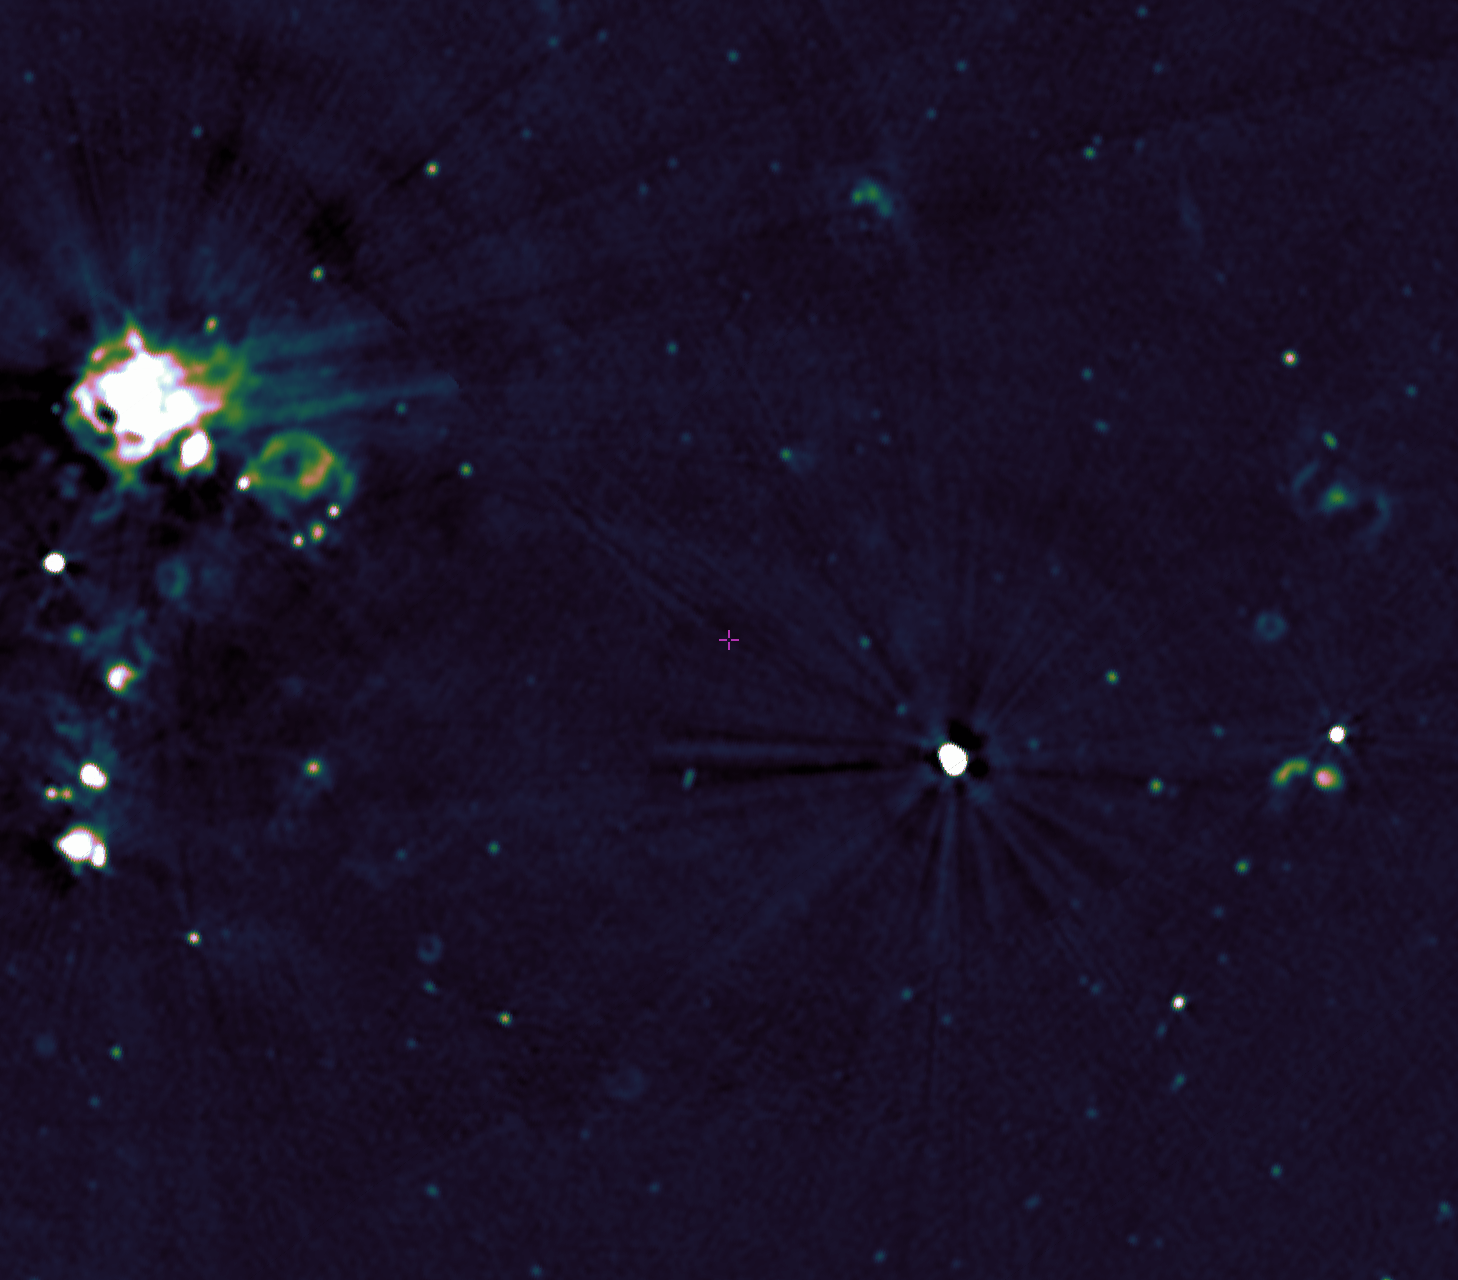
\includegraphics[width=0.40\linewidth]{./chapters/10.results/LMC/radio-843_cut.png}
	\caption{Large Magellanic Cloud shown in optical and radio wavelengths}
	\label{results:radio}
\end{figure}

\cite{bock1999sumss} sumss radio survey with the VLA radio interferometer.


	
\begin{figure}[h]
	\centering
	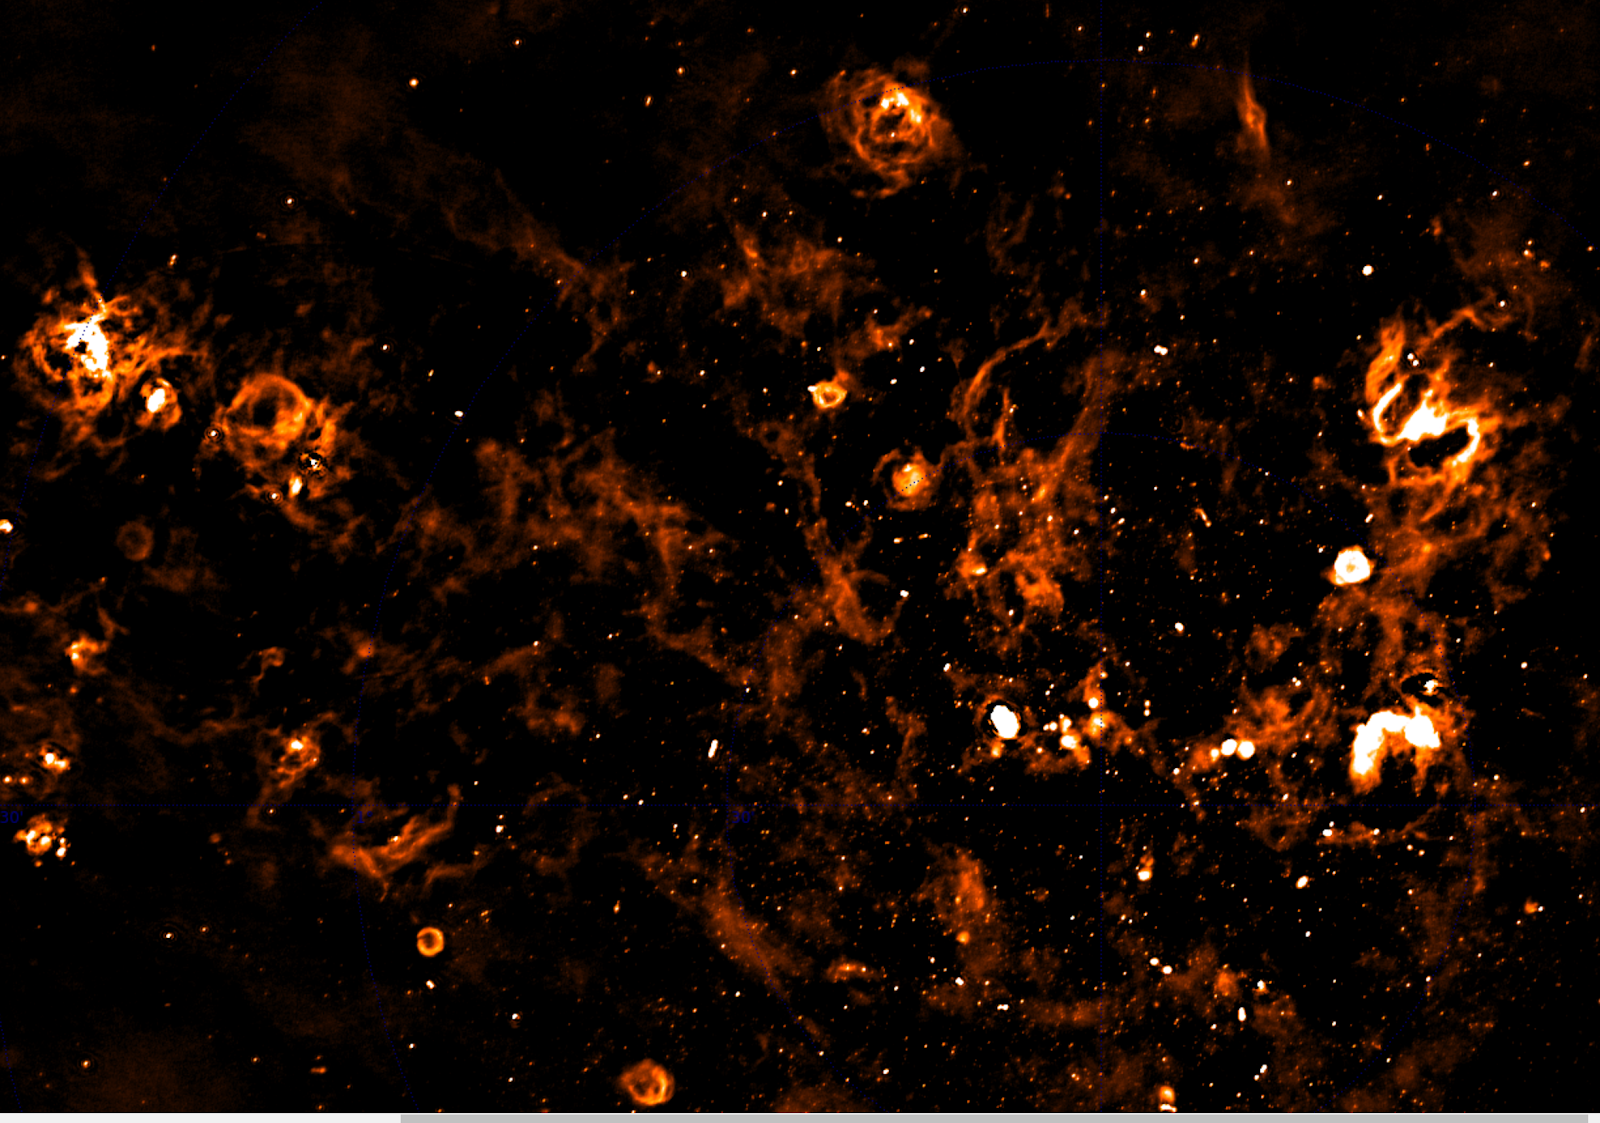
\includegraphics[width=0.80\linewidth]{./chapters/10.results/LMC/meerkat.png}
	\caption{Radio interferometer system}
	\label{results:radio}
\end{figure}

The problems: wide field of view, wide-band, and polarization. Full data

Too big.



\subsection{Comparison with CLEAN reconstruction}

\subsection{GPU Acceleration}

\subsection{Distributed coordinate descent}




\subsection{Wall clock time}
\begin{figure}[h]
	\centering
	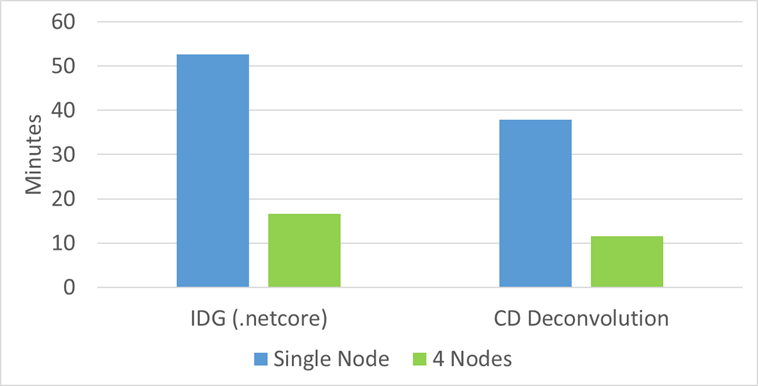
\includegraphics[width=0.80\linewidth]{./chapters/10.results/wall-clock-time.png}
	\caption{Wall-clock time of the distributed reconstruction}
	\label{results:time:fig}
\end{figure}


\subsection{Validity of gradient approximation} \label{results:gradients}

\begin{figure}[h]
	\centering
	\begin{subfigure}[b]{1.0\linewidth}
		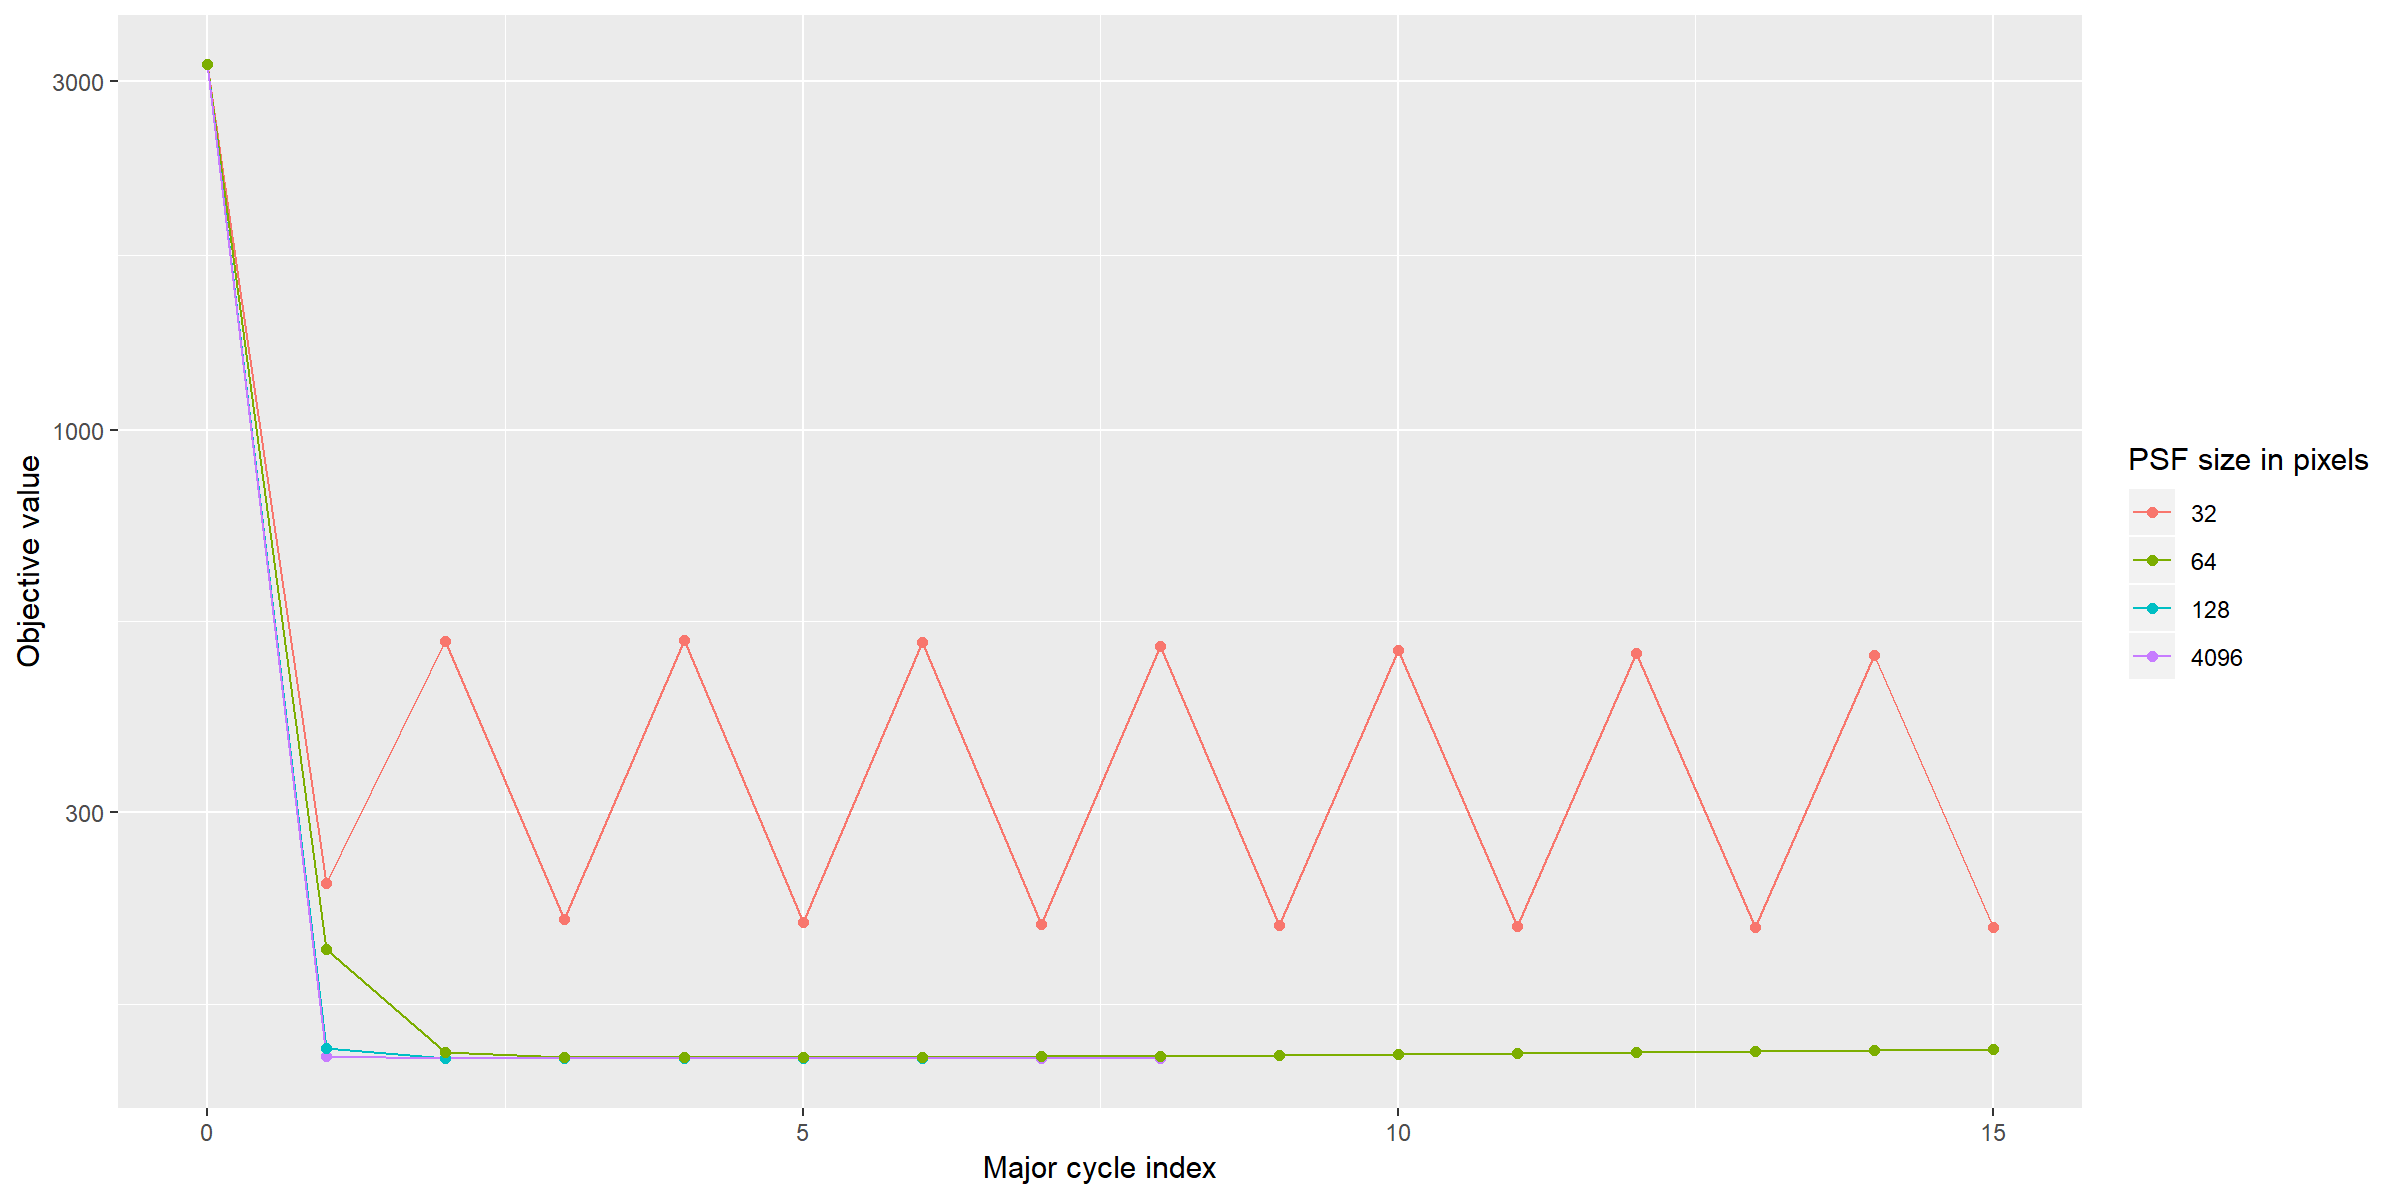
\includegraphics[width=\linewidth]{./chapters/10.results/gradient/size.png}
	\end{subfigure}
	
	\caption{Effect of the L1 and L2 Norm separately.}
	\label{results:gradients:size}
\end{figure}

\begin{figure}[h]
	\centering
	\begin{subfigure}[b]{1.0\linewidth}
		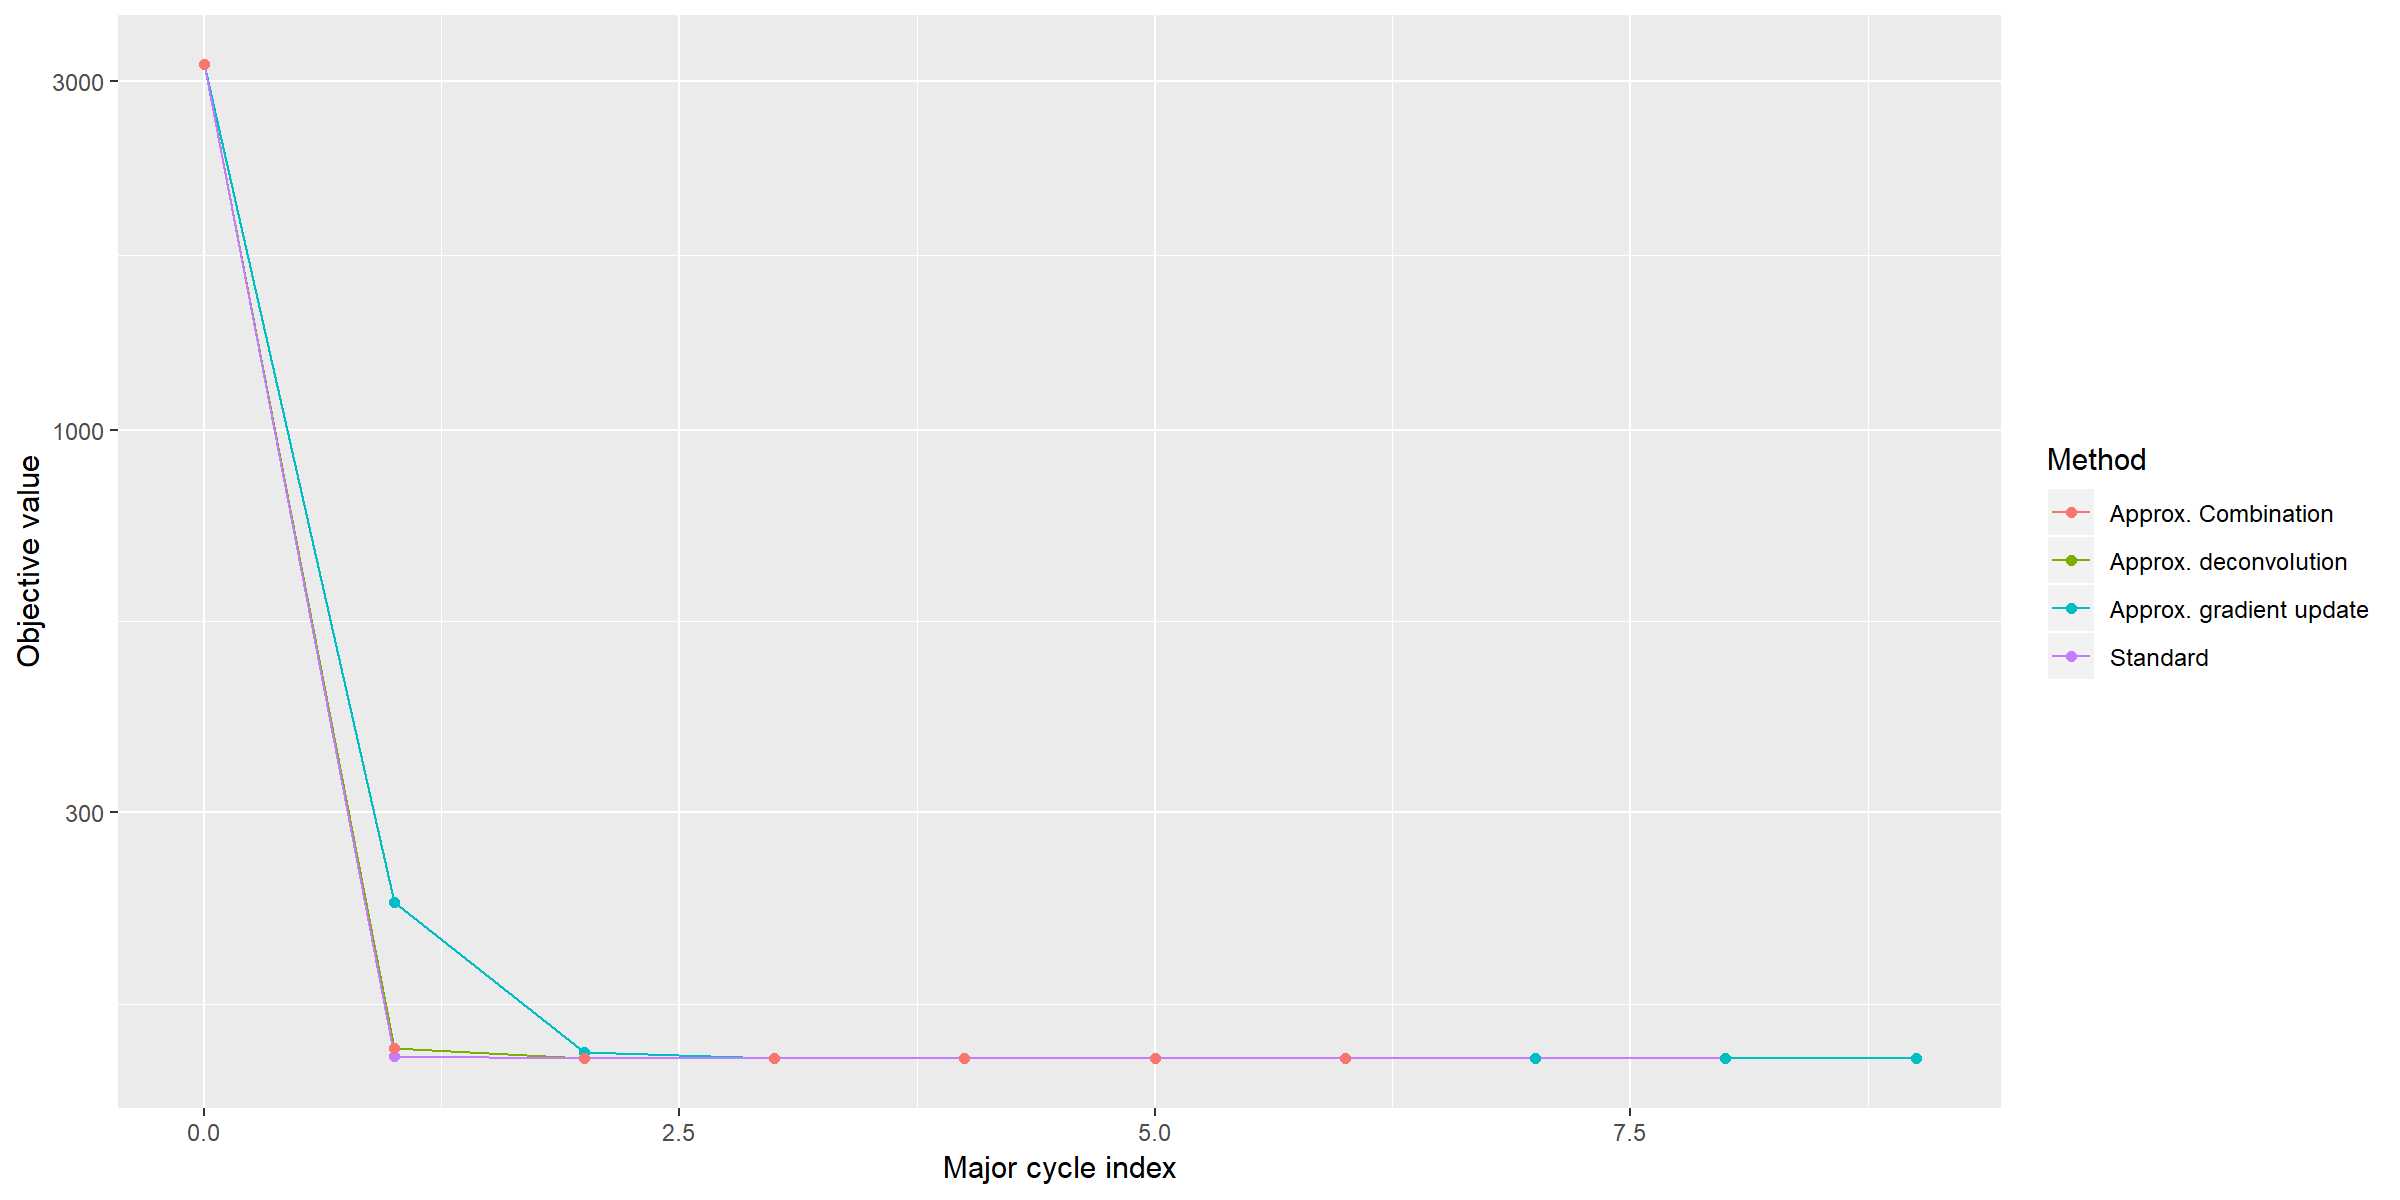
\includegraphics[width=\linewidth]{./chapters/10.results/gradient/comparison.png}
	\end{subfigure}
	\begin{subfigure}[b]{1.0\linewidth}
		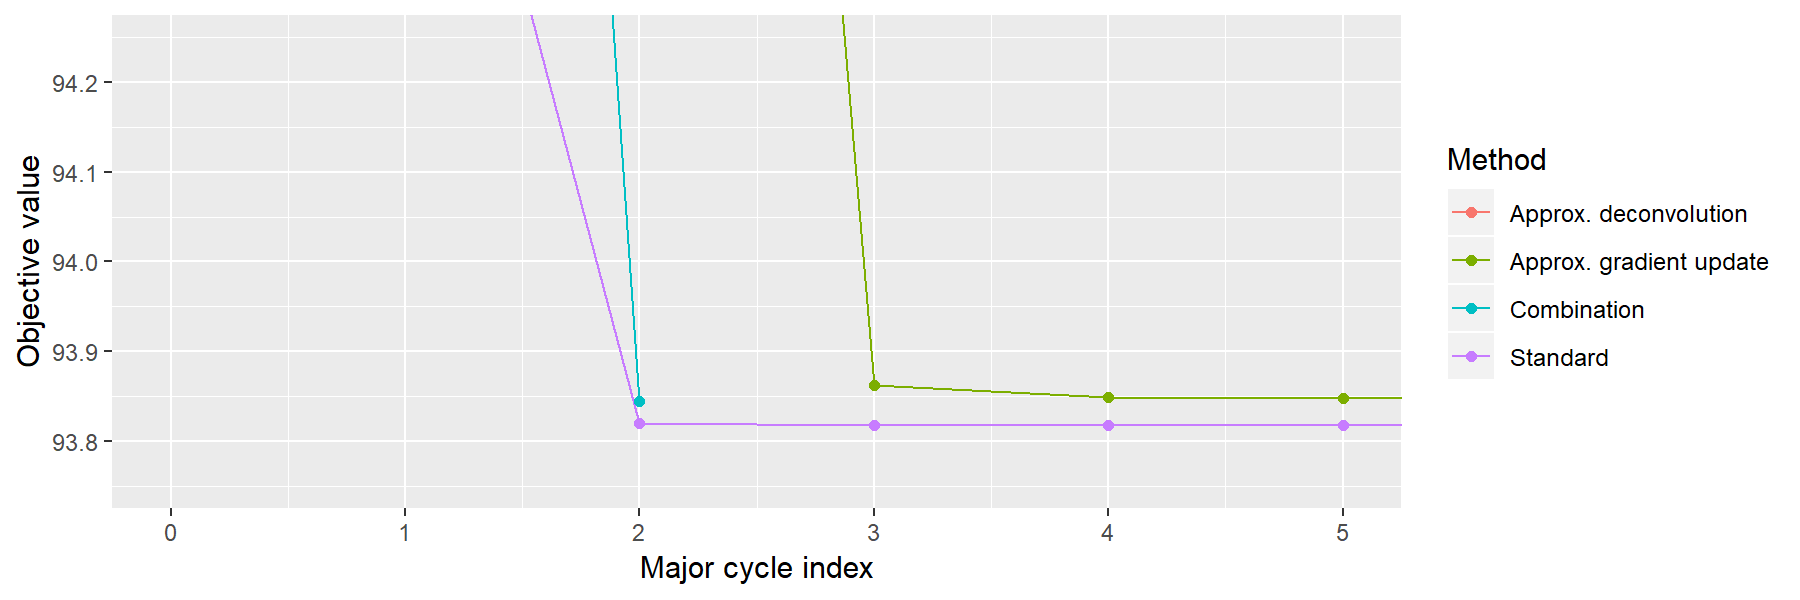
\includegraphics[width=\linewidth]{./chapters/10.results/gradient/comparison_zoom.png}
	\end{subfigure}
	
	\caption{Effect of the L1 and L2 Norm separately.}
	\label{results:gradients:comparison}
\end{figure}